%For example, the rapid growth of dataset\ion{What is "dataset" here?} and machine learning model sizes has driven recent work exploring efficient broadcast deployment of large models to geo-distributed regions \cite{sima2022ekko} \cite{flinn2022owl}.~\ion{Aren't regions geo-distributed (at different geo locations) by definition?}
% As a consequence, many cloud providers now offer data broadcast services~\cite{something} to simplify these common data movement tasks. 

%% Other motivations for broadcast that joey cut
%  Also, ML models often must be deployed to multiple geo-distributed regions to serve predictions with sufficiently low latency (e.g. Ekko). 
% A machine learning model trained on recent data should ideally be propagated to serving regions with very low latency (cite: Ekko).


% In addition, differentiated services across cloud providers creates an opportunity to utilize multiple cloud providers (e.g. GCP, Azure, Cloudflare, etc.) to reduce cost and improve service quality. %% Joey: I don't think we need the "sky" thesis to support ths paper so why bring it up in the intro

% Similarly, new satellite image data uploaded to a single cloud region may need to be shared with researchers processing data both in different regions or using different cloud providers. 






%Selecting the
% , deploying, and managing 
%the optimal overlay configuration across multiple public clouds presents a new set of challenges.
% system design challenges. 

% Skyplane\cite{} explored the use of this ephemeral overlay routing to minimize point-to-point data trasnfers but did not study the problem of data broadcast. 


% For example, Skyplane uses overlay networks to route data long throughput-maximizing overlay networks for point-to-point transfers. 


%,  the path that data is routed and not the associated bandwidth or routing resources.



% data broadcast in the cloud also introduces a unique opportunity to leverage elasticity to control the route data takes.  
% % The \emph{``fast is cheap''} mantra that drives many cloud applications implies that we can cheaply increase bandwidth by adding VMs to route broadcast traffic. 
% % Data broadcast in the cloud also offers several unique opportunities. 
% First, because there are on the order of a few thousand regions across the major cloud providers, the broadcast problem can be solve in a more centralized fashion.  
% Second, the elasticity of the cloud enables us to launch 

%Lastly, the specifics of the pricing models, as well as resource limits, can vary by orders of magnitude across cloud providers.








% \begin{figure}[t]
%     \centering
%     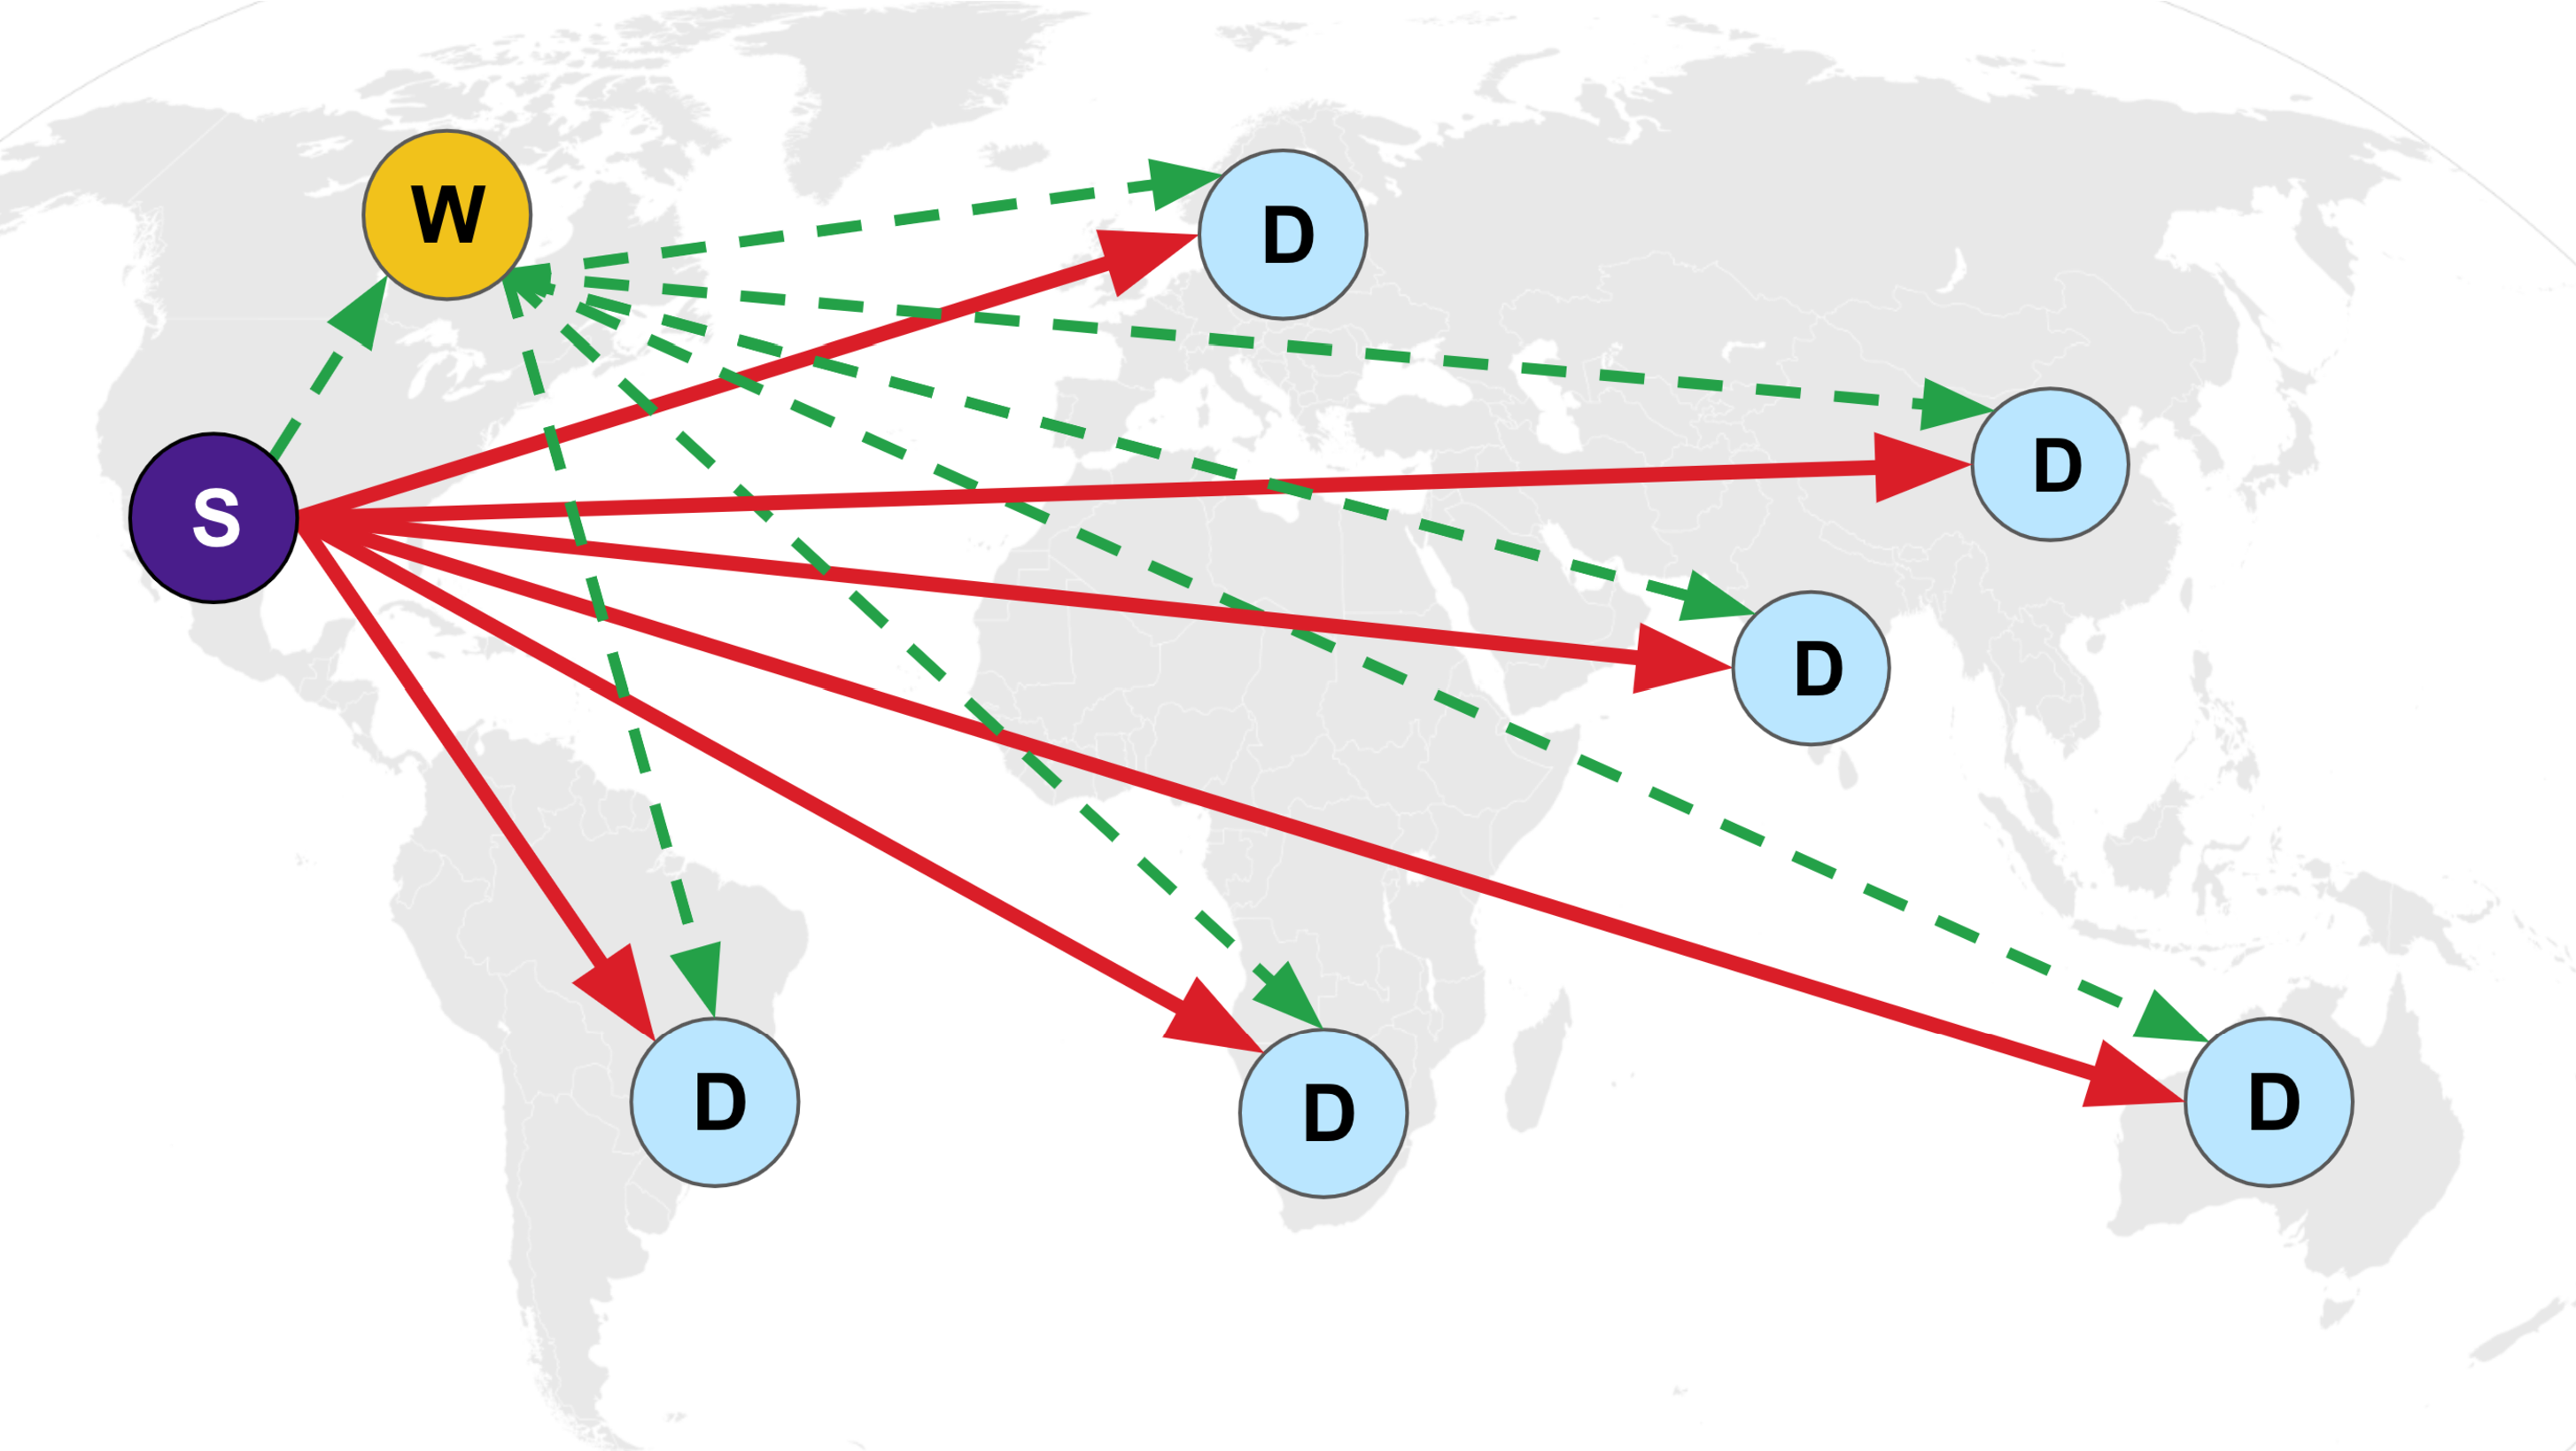
\includegraphics[width=\linewidth]{figures/overview.pdf}
%     \caption{\textbf{Overview of data broadcast with \sys.} \sys creates an overlay network using cloud VMs to route through cloud providers and cloud regions to optimize for throughput and cost. The \textit{overlay path} routes data through a region that is neither a source nor destination region but improves the topology's throughput and/or cost.}
%     \label{fig:overview}
% \end{figure}





%Given a source and set of destination cloud regions, \sys determines an optimal overlay topology, deploys an ephemeral overlay network, and routes traffic over the network to all destination nodes.
% At a high level, \sys allows users to ingest data at a source region using a modular set of connectors (e.g., a VM's filesystem or cloud object store) and broadcast it to one or more destination regions/providers.
%We study the design of several different optimization algorithms for determining the optimal overlay
% and introduce a simple extensible router architecture.




% Ion: provides a lot of flexbility in the cloud - e.g. how many machines 
% Ion: also have few destinations, unlike P2P (emphasize this more) 

%In this work, we consider the specific case of bulk data broadcast in the cloud, which introduces new dimensions to the traditional broadcast problem. First, nearly all cloud providers have a pricing model which incurs fees based on the amount of data transferred per GB. These fees are typically low (or even free) for data moving between regions within a single cloud. However, data movement \textit{out} of a cloud (i.e. data egress) is charged at higher rates. 
% Ion: does this matter for the algorithms? Potentially remove. 
%Second, cloud providers have their own intra-cloud networking, which often offers much better performance than in the traditional WAN context.

%Optimizing throughput and price of cloud transfers can be complex, as cloud providers have a surprising amount of heterogeneity in their network offerings, both in terms of performance and pricing. Different cloud providers impose different limits on per-instance bandwidth.
%In addition, there is variability in network performance between different region pairs both within and between cloud providers.
%For example, Azure networks (have higher performance? is this consistent for all regions?)
%For pricing, most providers follow similar pricing models that charge per GB of data moved between regions or in and out of the cloud provider (data ingress and egress, respectively), though exact pricing varies across providers.
%Data moved \textit{out} of the cloud provider (i.e. data egress) is charged at a higher rate to encourage users to keep their data within the cloud.
%Smaller providers are incentivized to compete on price, e.g., Cloudflare, which offers free egress to other clouds.
%As such, identifying cost-efficient ways to broadcast data through one or more clouds requires modeling these pricing discrepancies resulting from different business strategies.





%In this paper, we present \sys{}, a tool for bulk data broadcast with flexible broadcast topologies implemented over an overlay network.
%\sys{} contains an optimizer that uses a cost model of inter- and intra-cloud data transfer and throughput profiles of cloud networks to estimate the cost and throughput of different broadcast topologies.
%We implement several classical algorithms on top of \sys{} as well as a novel ILP program to minimize cost under throughput constraints.  
%We compare \sys{} with both open-source baselines (BitTorrent) and commercial offerings: specifically, multi-region replication offered by cloud providers. We show that \sys{} can outperform existing systems in both cost and throughput metrics while allowing these metrics to be flexibly traded off depending on the ILP parameters or the topology algorithm. 


% Ion: provides a lot of flexbility in the cloud - e.g. how many machines 
% Ion: also have few destinations, unlike P2P (emphasize this more) 

% NOTE: we should discuss why the ILP is intractable - the necessity of the approximations (volume, rather than throughput based - pricing of the volume) This creates weird scenarios where adding more resources reduces cost. 

 % TODO: end with emphaiszing throughput better - can use cost savings to get higher throughput (more VMs) 

 % bandwidth is cheap (fast is cheap) but VOLUME is expensive 

 % data has an identify - cannot use flow formulation 

 % volume and zero egress are fundamentally interesting 

% don't make it skyplane + broadcast - specifically models in terms of VOLUME not throughput 

% add discussion sesion - what if X 

